\hypertarget{pourquoi-laravel}{%
\section{\texorpdfstring{Pourquoi \href{https://laravel.com/}{Laravel}
?}{Pourquoi Laravel ?}}\label{pourquoi-laravel}}

\begin{itemize}
\tightlist
\item
  Framework full stack / glue
\item
  Prise en main rapide
\item
  Bonne documentation, grande \href{http://laravel.io/forum}{communauté}
\item
  Incite au respect des principes
  \href{http://fr.wikipedia.org/wiki/SOLID_(informatique)}{S.O.L.I.D}
\item
  Gratuit et opensource (Licence MIT)
\end{itemize}

\hypertarget{historique}{%
\section{Historique}\label{historique}}

\begin{itemize}
\tightlist
\item
  Projet initié en 2011 par \href{http://taylorotwell.com/}{Taylor
  Otwell}
\item
  Basé sur des composants d'autres frameworks
\item
  Mai 2013 : version 4, utilise
  \href{https://getcomposer.org/}{composer}
\item
  Août 2014 : projet PHP le plus
  \href{https://github.com/search?l=PHP\&q=stars\%3A\%3E0\&ref=searchresults\&type=Repositories}{populaire}
  sur github
\item
  \href{https://madewithlaravel.com/}{Qui} utilise Laravel ?
\item
  version 9 publiée 08.02.22, v10 : 07.02.23
\end{itemize}

\hypertarget{principales-fonctionnalituxe9s}{%
\section{Principales
fonctionnalités}\label{principales-fonctionnalituxe9s}}

\begin{itemize}
\tightlist
\item
  Routes RESTful
\item
  ORM (Eloquent, implémentation du pattern Active Record)
\item
  Migrations
\item
  Moteur de templates (Blade)
\item
  Pagination
\item
  Authentification, sessions
\item
  Mail
\item
  Tests unitaires
\item
  Extensible par \href{http://packalyst.com/}{packages} (bundles) via
  composer
\end{itemize}

\hypertarget{le-front-controller}{%
\section{Le Front Controller}\label{le-front-controller}}

\begin{figure}
\centering
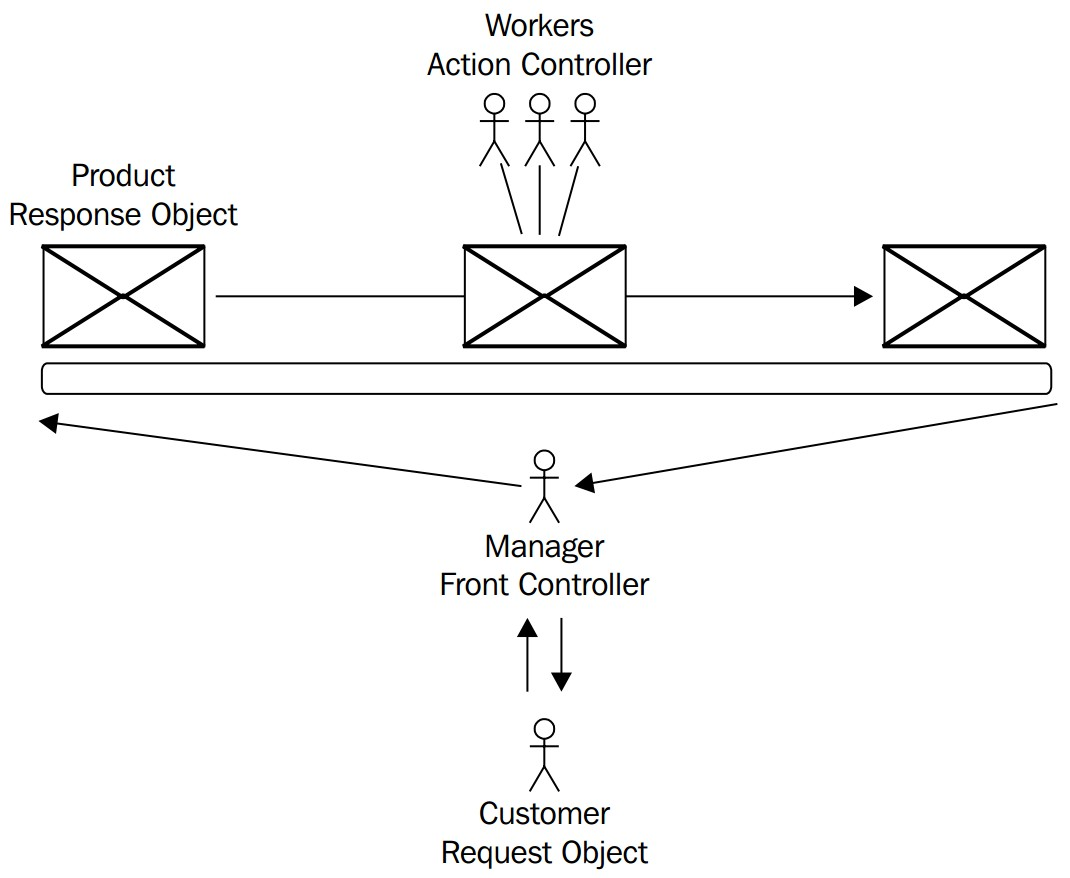
\includegraphics{src/img/front-ctrl.jpg}
\caption{Rôle du front controller}
\end{figure}

\hypertarget{architecture}{%
\section{Architecture}\label{architecture}}

\begin{figure}
\centering
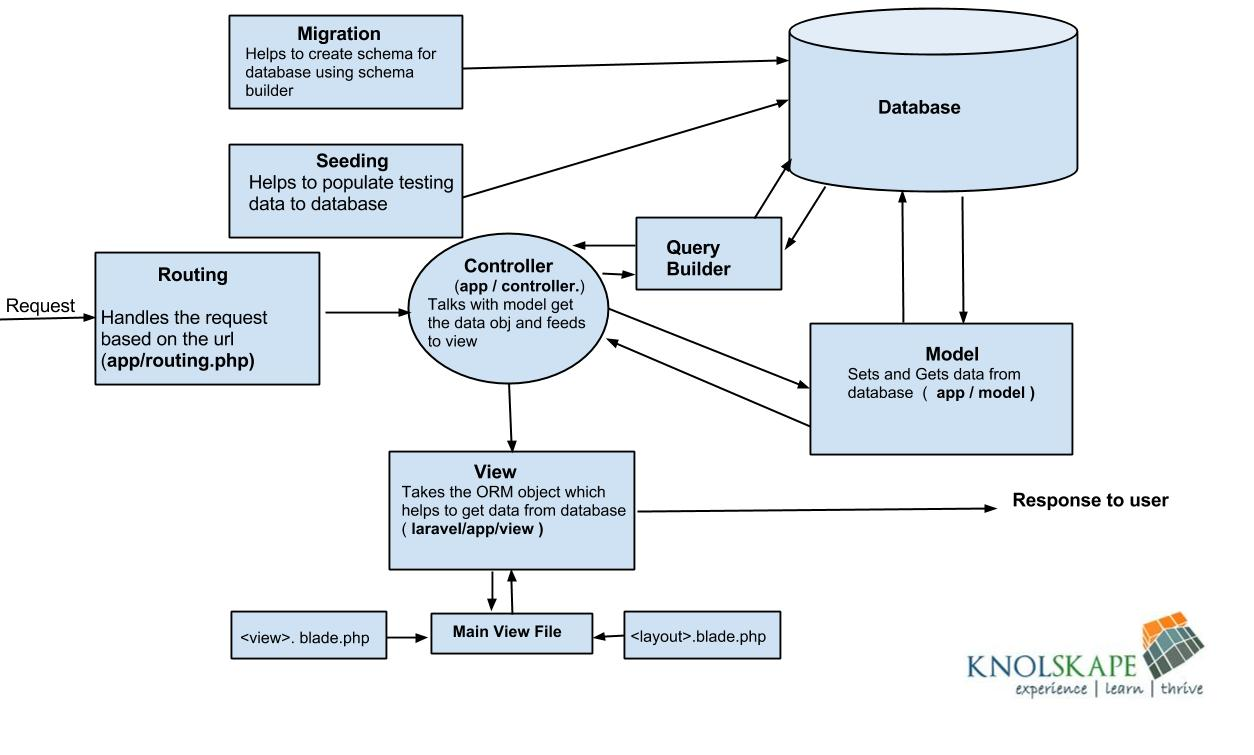
\includegraphics{src/img/laravel-architecture.jpg}
\caption{Architecture de Laravel}
\end{figure}

\hypertarget{mvc}{%
\section{MVC}\label{mvc}}

\begin{itemize}
\tightlist
\item
  Structure d'une appli web =
  \href{https://laravel.com/docs/master/lifecycle}{cycle
  Requête/Reponse}
\item
  Modèle : Eloquent ORM
\item
  Vue : Blade Engine
\item
  Contrôleur : hérite de BaseController
\end{itemize}

\hypertarget{pratique}{%
\section{Pratique}\label{pratique}}

\begin{itemize}
\tightlist
\item
  Conventions de codage : Laravel respecte
  \href{https://laravel.com/docs/5.1/contributions\#coding-style}{PSR-2}

  \begin{itemize}
  \tightlist
  \item
    Vous aussi avec \href{https://styleci.io/}{StyleCI}
  \end{itemize}
\item
  Editeurs et IDE : PhpStorm, \href{https://glitch.com/}{glitch},
  brackets, VS Code, \href{https://repl.it/}{repl.it},
  \href{https://www.gitpod.io/}{Gitpod}\ldots{}
\item
  Tests : unitaires, Jmeter, Selenium, \ldots{}
\item
  Outils : devtools Chrome ou FF, \href{http://emmet.io/}{Emmet}, git
\item
  Doc

  \begin{itemize}
  \tightlist
  \item
    \href{https://laravel.com/docs/master}{Documentation officielle} de
    Laravel
  \item
    Cheat Sheet \href{https://learninglaravel.net/cheatsheet/}{Laravel
    8}, \href{https://artisan.page/}{Artisan 9}
  \end{itemize}
\item
  Tutoriels

  \begin{itemize}
  \tightlist
  \item
    Pour un tuto à jour : bien préciser la version (8) dans votre
    recherche
  \item
    Laravel 9 : \href{https://laravel.sillo.org/laravel-9/}{Best Momo},
    \href{https://www.tutsmake.com/page/1/?s=tutorial+laravel+9}{Tuts
    Make},
    \href{https://www.pluralsight.com/courses/laravel-9-fundamentals}{Plural
    Sight}
  \end{itemize}
\end{itemize}

\hypertarget{environnement-de-duxe9veloppement}{%
\section{Environnement de
développement}\label{environnement-de-duxe9veloppement}}

\begin{itemize}
\tightlist
\item
  De quoi ai-je besoin pour développer ?

  \begin{itemize}
  \tightlist
  \item
    (L)AMP : Serveur HTTP, SGBD, PHP
  \item
    Git
  \item
    \href{https://getcomposer.org/}{Composer} : gestionnaire de
    dépendances PHP
  \item
    Associer nom de domaine au dossier projet
  \end{itemize}
\item
  Installer Laravel (créer un nouveau projet)
\end{itemize}

\begin{english}

\begin{Shaded}
\begin{Highlighting}[]
\VariableTok{$composer} \ExtensionTok{global}\NormalTok{ require }\StringTok{"laravel/installer"}
\end{Highlighting}
\end{Shaded}

\end{english}

\begin{itemize}
\tightlist
\item
  Le déploiement est simplifié si l'env de \textbf{dev} ressemble à
  celui de \textbf{production}
\end{itemize}

\hypertarget{environnement-de-duxe9veloppement-1}{%
\section{Environnement de
développement}\label{environnement-de-duxe9veloppement-1}}

\begin{itemize}
\tightlist
\item
  Local

  \begin{itemize}
  \tightlist
  \item
    Installation AMP, git + configuration : Long
  \item
    Dépendant du poste de travail
  \item
    Travail offline
  \end{itemize}
\item
  VM (Vagrant -
  \href{https://laravel.com/docs/master/homestead}{Homestead}) ou
  conteneur

  \begin{itemize}
  \tightlist
  \item
    Mise en route plus rapide : pré-configuré
  \item
    Environnement dédié au dev, identique pour chaque développeur
  \end{itemize}
\item
  Cloud (koding.com, coder.com, repl.it, gitpod \ldots)

  \begin{itemize}
  \tightlist
  \item
    Mise en route plus rapide : pré-configuré
  \item
    Indépendant du poste de travail (navigateur)
  \item
    Outils de synchro disponibles
  \end{itemize}
\end{itemize}

\hypertarget{aide-uxe0-la-mise-en-place-du-dev-env}{%
\section{Aide à la mise en place du dev
env}\label{aide-uxe0-la-mise-en-place-du-dev-env}}

\begin{itemize}
\tightlist
\item
  Paquets AMP (WAMP, EasyPHP, \ldots)
\item
  Pour aller plus vite :

  \begin{itemize}
  \tightlist
  \item
    Windows : \href{https://laragon.org/}{Laragon}
  \item
    Laravel Valet pour
    \href{https://laravel.com/docs/master/valet}{Mac},
    \href{https://cpriego.github.io/valet-linux/\#installation}{Ubuntu},
    et \href{https://github.com/valeryan/valet-wsl}{WSL}
  \end{itemize}
\item
  Windows avec WSL

  \begin{itemize}
  \tightlist
  \item
    \href{https://jackwhiting.co.uk/posts/setting-up-a-windows-10-development-environment-with-wsl-php-laravel/}{Tuto}
  \end{itemize}
\end{itemize}

\hypertarget{duxe9marrer-un-projet}{%
\section{Démarrer un projet}\label{duxe9marrer-un-projet}}

\begin{itemize}
\tightlist
\item
  Créer un nouveau projet
\end{itemize}

\begin{english}

\begin{Shaded}
\begin{Highlighting}[]
\NormalTok{$ }\ExtensionTok{composer}\NormalTok{ create{-}project laravel/laravel raidit}
\CommentTok{\# ou si \textasciitilde{}/.composer/vendor/bin est dans le PATH :}
\NormalTok{$ }\ExtensionTok{laravel}\NormalTok{ new raidit}
\NormalTok{$ }\BuiltInTok{cd}\NormalTok{ raidit}
\end{Highlighting}
\end{Shaded}

\end{english}

\begin{itemize}
\tightlist
\item
  Racine du site dans \textenglish{\texttt{/public}} (lien symbolique ou
  virtual host)
\end{itemize}

\hypertarget{le-duxe9puxf4t}{%
\section{Le dépôt}\label{le-duxe9puxf4t}}

\begin{itemize}
\tightlist
\item
  Initialiser le dépôt
\end{itemize}

\begin{english}

\begin{Shaded}
\begin{Highlighting}[]
\VariableTok{$cd} \ExtensionTok{raidit}
\VariableTok{$git} \ExtensionTok{init}
\VariableTok{$git} \ExtensionTok{add}\NormalTok{ .}
\VariableTok{$git} \ExtensionTok{commit}\NormalTok{ {-}m }\StringTok{"Install laravel"}
\VariableTok{$git} \ExtensionTok{remote}\NormalTok{ add origin git@github.com:bastian/raidit.git}
\VariableTok{$git} \ExtensionTok{push}\NormalTok{ {-}{-}set{-}upstream origin master}
\end{Highlighting}
\end{Shaded}

\end{english}

\begin{itemize}
\tightlist
\item
  Penser à ajouter sa clé publique à Github
\end{itemize}

\hypertarget{apache}{%
\section{Apache}\label{apache}}

\begin{itemize}
\tightlist
\item
  Virtual hosts

  \begin{itemize}
  \tightlist
  \item
    \textenglish{\texttt{http-vhosts.conf}} (activer dans
    \textenglish{\texttt{httpd.conf}})
  \item
    Un par site
  \item
    Pointer dans \textenglish{\texttt{/public}}
  \end{itemize}
\item
  \textenglish{\texttt{AllowOverride}} : active
  \textenglish{\texttt{.htaccess}}
\item
  \textenglish{\texttt{.htaccess}} : redirection des requêtes
\item
  Alternative : Remplacer le dossier racine http par un lien symbolique
  vers le dossier \textenglish{\texttt{/public}}
\end{itemize}

\hypertarget{artisan}{%
\section{Artisan}\label{artisan}}

\begin{itemize}
\tightlist
\item
  Laravel's CLI
\item
  Construit avec Symfony Console
\item
  Aide aux tâches courantes, ex:
\end{itemize}

\begin{english}

\begin{Shaded}
\begin{Highlighting}[]
\VariableTok{$php} \ExtensionTok{artisan}\NormalTok{ route:list}
\VariableTok{$php} \ExtensionTok{artisan}\NormalTok{ migrate}
\VariableTok{$php} \ExtensionTok{artisan}\NormalTok{ make:controller}

\VariableTok{$php} \ExtensionTok{artisan}\NormalTok{ list}
\end{Highlighting}
\end{Shaded}

\end{english}

\begin{itemize}
\tightlist
\item
  \href{https://laravel.com/docs/master/artisan}{Extensible}
\end{itemize}

\hypertarget{premiers-pas}{%
\section{Premiers pas}\label{premiers-pas}}

\begin{itemize}
\tightlist
\item
  \href{https://laravel.com/docs/master/routing}{Routes}

  \begin{itemize}
  \tightlist
  \item
    Ajouter une route \textenglish{\texttt{/test}}
  \item
    Ajouter un paramètre qui sera affiché :
    \textenglish{\texttt{/test/param}}
  \item
    Utiliser une vue pour cette route
  \item
    Lister les routes avec la commande artisan
  \end{itemize}
\end{itemize}

. . .

\begin{itemize}
\tightlist
\item
  \href{https://laravel.com/docs/master/controllers}{Contrôleurs}

  \begin{itemize}
  \tightlist
  \item
    Ajouter un contrôleur : \textenglish{\texttt{Test}}
  \item
    Lui ajouter une action : \textenglish{\texttt{index}}
  \item
    Ajouter la route correspondante : \textenglish{\texttt{/test/index}}
  \end{itemize}
\end{itemize}

. . .

\begin{itemize}
\tightlist
\item
  \href{https://laravel.com/docs/master/views}{Vues}

  \begin{itemize}
  \tightlist
  \item
    Ajouter une vue Blade (\textenglish{\texttt{.blade.php}})
  \item
    Afficher cette vue dans l'action \textenglish{\texttt{index}}
  \end{itemize}
\end{itemize}

\hypertarget{ressources}{%
\section{Ressources}\label{ressources}}

\begin{itemize}
\tightlist
\item
  \href{https://github.com/LaravelDaily/laravel-tips}{Tips}
\item
  \href{https://hackr.io/blog/laravel-cheat-sheet}{Cheat Sheet}
\item
  \href{https://laracasts.com/search?query=laravel\%209}{Laracast}
\item
  \href{http://learninglaravel.net/tags/tutorials}{Learning Laravel}
\item
  \href{https://www.tutsmake.com/laravel-8-rest-api-crud-with-passport-auth-tutorial/}{Laravel
  REST API CRUD tuto}
\item
  \href{https://github.com/HE-Arc/slides-devweb/wiki/Ressources}{Les
  vôtres}
\end{itemize}

\hypertarget{sources}{%
\section{Sources}\label{sources}}
